\thepage
\section{Introduction}

%- No collocation
%- Enterprise support
%- Version control, issue tracking

In recent years open source software solutions have become widely popular and frequently used in both scientific and enterprise use, which can be attributed to a number of factors, most importantly the ease of development and deployment of IT projects, improved cybersecurity and enhanced scalability \cite{pwcLeadingBenefitsOpensource2016}. This increases the contribution to open source projects from enterprises and individuals alike. Due to its nature, open source software projects are driven by community contributions, and depend heavily on active participation in all phases of the project. \\

Software development in a corporate environment usually follows a strict hierarchial structure, where each participant is given a precise position and responsibility, like project manager, scrum master, senior or junior developer, and employees do not tend to work outside of their assigned tasks and territories. The main purpose of maintaining software development structures is for the company to ensure that the outcome of the project is in accordance with the business objective, adheres to the pre-set quality criteria and it is completed in a given timeframe; in other words to asses the risks associated with the business objective of the software project \cite{surekaUsingSocialNetwork2011}. This is achieved by breaking down the developed software into smaller, less complex components, and grouping the developers into managable teams, where the communication is moderated between teams \cite{birdLatentSocialStructure2008}. \\

% Open-source software development properties
As opposed to commercial software development, Free/Libre Open Source Software (FLOSS) projects usually do not follow an organizational hierarchy, and are usually self-organizing and dynamic \cite{birdLatentSocialStructure2008}. Issues, bugs and progress are tracked openly, and everyone is encouraged to contribute based on the current topics and expertise, but purely on a volunteering basis. The lack of access restriction to certain modules allows for much more spontaneous interaction between developers, which generate large, complex networks \cite{martinez-romoUsingSocialNetwork2008}. These complex networks can be seen as large social networks of developers based on collaboration. \\

% AUTHOR NAME HARDCODED HERE
Because contribution to FLOSS projects are voluntary, participants have a different motivation for taking part than in commercial software development. According to El Asir et al. \cite{elasriPeripheryCoreTemporal2017}, FLOSS participation can be motivated by internal and external factors. Internal factors include self-improvement, learning and contribution as a hobby or pass-time activity  \cite{alexanderharsWorkingFreeMotivations2002,yunwenyeUnderstandingMotivationOpen2003}, whereas external factors are motivated by marketing and demonstrating certain skills, thus increasing and improving employability \cite{alexanderharsWorkingFreeMotivations2002}. \\

% Summary of background literature and state of the art solutions
\section{Background and rationale}

\subsection{Collaboration in FLOSS projects}
% - FLOSS definition
% AUTHOR NAME HARDCODED HERE
Collaboration networks of open source software (OSS) have been a subject of many academic research. Raymond \cite{crowstonSocialStructureFree2005} has defined collaboration based on bug report interaction, and observed the collaboration network of 124 large-scale SourceForge projects. The generated networks have widely different centralization properties, but it was observed that larger sized projects tend to be more decentralized. The broad community roles contributors tend to take have been also identified in \cite{crowstonSocialStructureFree2005}, which have been coined as the \textit{onion model} in \cite{martinez-romoUsingSocialNetwork2008} (Figure \ref{fig:onion1}). \\

\begin{figure}
    \centering
    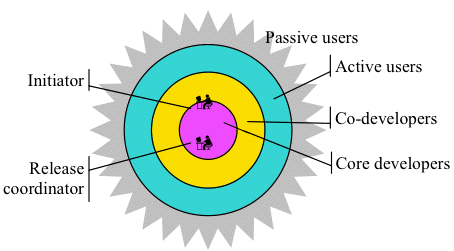
\includegraphics[width=0.6\textwidth]{figures/onion_model.png}
    \caption{Onion model of collaboration types in FLOSS projects \cite{crowstonSocialStructureFree2005}.}
    \label{fig:onion1}
\end{figure}

The onion model describes the types of participants in an OSS project as layers. The center represents the small group of core developers, who are responsible for the majority of contributions to the software. They are surrounded by a larger group of co-developers, whose main contributions are usually bug fixes reported by the active users. The passive users are usually the largest in numbers, who do not contribute or report any bugs. In a healthy FLOSS project, each layer of contributors are about one magnitude larger in numbers than the preceeding inner layer \cite{mockusTwoCaseStudies2002}. \\

% AUTHOR NAME HARDCODED HERE
El Asir et al. \cite{elasriPeripheryCoreTemporal2017} used a K-means classification to categorise project participants into a similar core-periphery structure (core, gray in-between area, and periphery) based on SNA metrics with a montly timeframe, and analysed how and why contributors transition between groups. They found that technical contributions like code commits and lines added have a much heavier impact on becoming a core developer as opposed to other activities, such as testing, reviewing and commenting. \\

% AUTHOR NAME HARDCODED HERE
A literature review conducted by McClean et al. \cite{mccleanSocialNetworkAnalysis2021} systematically analysed the state-of-the-art research of 46 scientific papers in the field of FLOSS social networks, and categorised them into three groups based on topic: structure, lifecycle and communication. They conclude, that the existence of core-periphery structure in OSS projects is well established in the field, which is also an indicator of a healthy FLOSS software. Regarding the lifecycle, generally the core development team does not change significantly over time, however, the project becomes more decentralised and distributed as it matures. A lack of research regarding temporal analyses were identified in the most current knowledge, which was suggested as a future research area in this field. \\

\subsection{Social network of Open-source projects}
\dots
%\begin{itemize}
%   \item Relevant social aspects of OS projects
%   \item State of the art
%   \item Collaboration by coediting files
%   \item Contributors form dynamic social networks
%    \item Problem of analysing changes over time in a network
%   \item Other studies in this field...
%\end{itemize}


\section{Motivation of research problem and research questions}
Because there is a high dependency on the community in open source software projects, by understanding how contributions are included and what patterns emerge we can gain valuable insight into the project's current state and its trajectory. As stated before, SNA analysis of OSS have been extensively studied, but there is a lack of research regarding temporal models analyzing the lifecycle of a FLOSS project. \\

The goal of this paper is to fill in this gap by examining OSS project collaboration networks over time using SNA metrics. More specifically, one part of the research will focus on the evolution of such collaboration networks and comparing and contrasting these networks with the software outcome. The second part will focus on events during a project, and how it affects the developer collaboration. The research questions, which are broken down into subquestions, are as follows:

\begin{enumerate}
    \item \textbf{How does the temporal lifecycle information of a project influence its success?} \\
    
    \begin{enumerate}
        \item \textit{Based on temporal models of collaboration, is it possible to predict the outcome of the project?} Since it has been proven that the core collaborators do not change much over the course of the OS software development, our assumption is that any sudden or long-term change, that is not consistent with the other observed projects, can have a significant impact on the outcome (negative or positive alike).
        \item \textit{Can stages of a FLOSS project with a maturity model be observed?} As most OS software starts with a small collaborator basis and grows over time, it can be assumed, that each project goes through the same steps of open source maturity levels. On the other hand, it is also possible that due to the uniqueness of each project, no such stages are observable. 
    \end{enumerate}

    \item \textbf{How do major events in the project lifecycle change the collaboration network of the project?}
    \begin{enumerate}
        \item \textit{Do planned or foreseeable events change the collaboration structure?} Major software version releases can be considered foreseeable events of the project lifecycle, which could have an effect on the developer collaboration. For example, there might be a higher rate of interaction between contributors just before a new version is released to clear up the backlog of tasks. But it is also possible, that commit and change rates drop during this time, because the focus shifts to stability and testing instead of new features.
        \item \textit{How unforeseeable internal or external events affect FLOSS collaboration?} Sudden shocks to the project, such as an announcement of disinterest from major users of the software, discontinued enterprise support of the project, large-scale global events like the pandemic, or sudden employee firings can have significant effect on the core and periphery collaborators alike. By analysing the collaboration network before, during and after such changes, we might be able to recognise patterns, that regularly occur around these events.
    \end{enumerate}
\end{enumerate}

\subsection{Research methodology}
To find answers to the research questions above, first we build a repository analyzer tool, which mines collaboration data from FLOSS projects, generates static snapshot collaboration networks at each given time interval and calculates SNA metrics for each snapshot. Then these metrics can be aggregated over time, or plotted against time to discover changes in the network. The \texttt{git2net}\footnote{\url{https://github.com/gotec/git2net}} \cite{goteAnalysingTimeStampedCoEditing2019} Python library provides the necessary tools to mine any project repository that uses git version control. It also incorporates temporal network generation capability, which can be used as a source for creating static collaboration networks aggregated over a given period of time. \\


We apply a hybrid methodology of qualitative and quantitative research. First, as part of the qualitative research, we choose a small number of repositories to be analyzed. We observe the number of connected components, centrality, number of nodes and mean degree SNA metrics in order to discover the core and peripherial collaborators over the project lifecycles. The basis of collaboration, due to the unavailability of other means of communication, is coediting files. Based on the state of the art research in this field, file coediting proves to be an effective and easy way to represent collaboration between developers. \\

After discovering the collaboration structure over time, we will match the breakpoints and unexpected spikes or troughs to events within the lifespan of the project. We expect that the key SNA metrics will show a periodicity around planned releases and other reoccurring events (e.g. holiday season). Outstanding values without reoccurrence, on the other hand, are more likely to be consequences of unexpected events. In these cases, it should be observed whether the network is capable of reorganizing itself, or does the event leave a permanent mark on the collaboration structure. A categorization of unexpected events and the level of impact each category has should be observed. \\

For the quantitative research to be conducted, we will gather a large set of repositories along with major events in its lifecycles. We will then run the miner for all repositories, and with the findings of the qualitative research, we will try to detect all major events and their type (planned or unexpected). We will utilize the \texttt{ruptures} \footnote{\url{https://github.com/deepcharles/ruptures}} library to detect changes in the continuous SNA metrics. If the model is capable to accurately recognise events, then we can also apply it on any repository to detect changes, which will allow us to discover changes in the collaboration network that are not related to publicly known events or releases. \\

% Quantitative research
% \begin{itemize}
%     \item Composing a large set of repositories (different sizes, properties) with their success or failure
%     \item Gathering major events for the repositories (version releases, external events, global events)
%     \item Detecting past changes automatically based on changes in measured statistics
%     \item How do changes and reoccurring patterns match the events?
%     \item What structures can be noticed before a major success or failure of a project?
% \end{itemize}


\section{Gitminer implementation}
% - what do we want to achieve with the gitminer
%  - generate networks of collaboration
%    - what should be the basis of collaboration
%  - filter for time
%  - generate statistics
\subsection{git2net miner}
% - git2net: database of commits and edits
% - repo_tools: release versions and tags

\subsection{Data cleaning and disambiguation}
% - issue of authors changing their names, having multiple identities
% - solution: first it was looking at email-name pairs, then: gambit
% - issue of special characters in node names --> replace with numbers
% - issue of same named files being merged
%  --> solution: remove duplicate files (rationale: these are mostly technical files)

\subsection{Collaboration networks}
% - Pathpy and networkx libraries

\subsubsection{Temporal networks}
% - preserves the time axis, but hard to visualize
% - snapshots are taken of the network, each edge only exist at a defined timestamp or timestamps
% - method of generating static networks
%(figure of a temporal network: subplots with timestamps visible)
\subsubsection{Static networks}
% - Easily visualizable
% - Looses time aspect, only considers a given period of time aggregated
% - Can be weighted
%    WOMP and weighted Jaccard methods (calculation, single nodes removed, etc...)
% (One WOMP and one Jaccard network)

\subsection{Graph statistics aggregation}
% - "Seeker" scanning over time
% - parameters: delta, interval, from, to
% - size of the project matters
% - activity determines the scale (less activity = small interval (week), vice versa)
% - helps: commits per day plot (insert)

\section{Collaboration pattern analysis}
\subsection{Observed projects and events}
% - which projects (Servo, pandas, numpy, networkx, seaborn, wasmtime, ruptures (?))
% - expected: Big releases
% - unexpected: layoffs
\subsection{SNA metrics analysis}
%....
\subsection{Results}
%....


% (\item Automatic event recognition)
%     (\item Event detection implementation (ruptures))
%     (\item Collaboration network change detection)
\section{Quantitative analysis of projects during crunch time}
\subsection{Collaboration network changes}
\subsection{Prediction of outcome based on collaboration changes}

\section{Discussion and results}
\section{Conclusion and future work}
